

%CUT AND PASTE THIS ENTIRE DOCUMENT INTO A BLANK DOCUMENT ON CloudSageMath. Then replace the content (title, name, and so on), with your stuff. If you have problems or errors, let me know!

%\documentclass[12pt]{amsart}
\documentclass{article}

\usepackage{tikz-cd}

%Python Code Listing
\usepackage[utf8]{inputenc}
\usepackage[english]{babel}
\usepackage[T1]{fontenc}

\usepackage{xcolor}
\definecolor{maroon}{cmyk}{0, 0.87, 0.68, 0.32}
\definecolor{halfgray}{gray}{0.55}
\definecolor{ipython_frame}{RGB}{207, 207, 207}
\definecolor{ipython_bg}{RGB}{247, 247, 247}
\definecolor{ipython_red}{RGB}{186, 33, 33}
\definecolor{ipython_green}{RGB}{0, 128, 0}
\definecolor{ipython_cyan}{RGB}{64, 128, 128}
\definecolor{ipython_purple}{RGB}{170, 34, 255}



\usepackage{listings}
\lstset{
   breaklines=true,
   %
   extendedchars=true,
   literate=
   {á}{{\'a}}1 {é}{{\'e}}1 {í}{{\'i}}1 {ó}{{\'o}}1 {ú}{{\'u}}1
   {Á}{{\'A}}1 {É}{{\'E}}1 {Í}{{\'I}}1 {Ó}{{\'O}}1 {Ú}{{\'U}}1
   {à}{{\`a}}1 {è}{{\`e}}1 {ì}{{\`i}}1 {ò}{{\`o}}1 {ù}{{\`u}}1
   {À}{{\`A}}1 {È}{{\'E}}1 {Ì}{{\`I}}1 {Ò}{{\`O}}1 {Ù}{{\`U}}1
   {ä}{{\"a}}1 {ë}{{\"e}}1 {ï}{{\"i}}1 {ö}{{\"o}}1 {ü}{{\"u}}1
   {Ä}{{\"A}}1 {Ë}{{\"E}}1 {Ï}{{\"I}}1 {Ö}{{\"O}}1 {Ü}{{\"U}}1
   {â}{{\^a}}1 {ê}{{\^e}}1 {î}{{\^i}}1 {ô}{{\^o}}1 {û}{{\^u}}1
   { }{{\^A}}1 {Ê}{{\^E}}1 {Î}{{\^I}}1 {Ô}{{\^O}}1 {Û}{{\^U}}1
   {œ}{{\oe}}1 {Œ}{{\OE}}1 {æ}{{\ae}}1 {Æ}{{\AE}}1 {ß}{{\ss}}1
   {ç}{{\c c}}1 {Ç}{{\c C}}1 {ø}{{\o}}1 {å}{{\r a}}1 {Å}{{\r A}}1
   {€}{{\EUR}}1 {£}{{\pounds}}1
}

%%
%% Python definition (c) 1998 Michael Weber
%% Additional definitions (2013) Alexis Dimitriadis
%% modified by me (should not have empty lines)
%%
\lstdefinelanguage{iPython}{
   morekeywords={access,and,break,class,continue,def,del,elif,else,except,exec,finally,for,from,global,if,import,in,is,lambda,not,or,pass,print,raise,return,try,while},%
   %
   % Built-ins
   morekeywords=[2]{abs,all,any,basestring,bin,bool,bytearray,callable,chr,classmethod,cmp,compile,complex,delattr,dict,dir,divmod,enumerate,eval,execfile,file,filter,float,format,frozenset,getattr,globals,hasattr,hash,help,hex,id,input,int,isinstance,issubclass,iter,len,list,locals,long,map,max,memoryview,min,next,object,oct,open,ord,pow,property,range,raw_input,reduce,reload,repr,reversed,round,set,setattr,slice,sorted,staticmethod,str,sum,super,tuple,type,unichr,unicode,vars,xrange,zip,apply,buffer,coerce,intern},%
   %
   sensitive=true,%
   morecomment=[l]\#,%
   morestring=[b]',%
   morestring=[b]",%
   %
   morestring=[s]{'''}{'''},% used for documentation text (mulitiline strings)
   morestring=[s]{"""}{"""},% added by Philipp Matthias Hahn
   %
   morestring=[s]{r'}{'},% `raw' strings
   morestring=[s]{r"}{"},%
   morestring=[s]{r'''}{'''},%
   morestring=[s]{r"""}{"""},%
   morestring=[s]{u'}{'},% unicode strings
   morestring=[s]{u"}{"},%
   morestring=[s]{u'''}{'''},%
   morestring=[s]{u"""}{"""},%
   %
   % {replace}{replacement}{lenght of replace}
   % *{-}{-}{1} will not replace in comments and so on
   literate=
   {á}{{\'a}}1 {é}{{\'e}}1 {í}{{\'i}}1 {ó}{{\'o}}1 {ú}{{\'u}}1
   {Á}{{\'A}}1 {É}{{\'E}}1 {Í}{{\'I}}1 {Ó}{{\'O}}1 {Ú}{{\'U}}1
   {à}{{\`a}}1 {è}{{\`e}}1 {ì}{{\`i}}1 {ò}{{\`o}}1 {ù}{{\`u}}1
   {À}{{\`A}}1 {È}{{\'E}}1 {Ì}{{\`I}}1 {Ò}{{\`O}}1 {Ù}{{\`U}}1
   {ä}{{\"a}}1 {ë}{{\"e}}1 {ï}{{\"i}}1 {ö}{{\"o}}1 {ü}{{\"u}}1
   {Ä}{{\"A}}1 {Ë}{{\"E}}1 {Ï}{{\"I}}1 {Ö}{{\"O}}1 {Ü}{{\"U}}1
   {â}{{\^a}}1 {ê}{{\^e}}1 {î}{{\^i}}1 {ô}{{\^o}}1 {û}{{\^u}}1
   { }{{\^A}}1 {Ê}{{\^E}}1 {Î}{{\^I}}1 {Ô}{{\^O}}1 {Û}{{\^U}}1
   {œ}{{\oe}}1 {Œ}{{\OE}}1 {æ}{{\ae}}1 {Æ}{{\AE}}1 {ß}{{\ss}}1
   {ç}{{\c c}}1 {Ç}{{\c C}}1 {ø}{{\o}}1 {å}{{\r a}}1 {Å}{{\r A}}1
   {€}{{\EUR}}1 {£}{{\pounds}}1
   %
   {^}{{{\color{ipython_purple}\^{}}}}1
   {=}{{{\color{ipython_purple}=}}}1
   %
   {+}{{{\color{ipython_purple}+}}}1
   {*}{{{\color{ipython_purple}$^\ast$}}}1
   {/}{{{\color{ipython_purple}/}}}1
   %
   {+=}{{{+=}}}1
   {-=}{{{-=}}}1
   {*=}{{{$^\ast$=}}}1
   {/=}{{{/=}}}1,
   literate=
   *{-}{{{\color{ipython_purple}-}}}1
    {?}{{{\color{ipython_purple}?}}}1,
   %
   identifierstyle=\color{black}\ttfamily,
   commentstyle=\color{ipython_cyan}\ttfamily,
   stringstyle=\color{ipython_red}\ttfamily,
   keepspaces=true,
   showspaces=false,
   showstringspaces=false,
   %
   rulecolor=\color{ipython_frame},
   frame=single,
   frameround={t}{t}{t}{t},
   framexleftmargin=6mm,
   numbers=left,
   numberstyle=\tiny\color{halfgray},
   %
   %
   backgroundcolor=\color{ipython_bg},
   %   extendedchars=true,
   basicstyle=\scriptsize,
   keywordstyle=\color{ipython_green}\ttfamily,
}

%%%%flowchart
\usetikzlibrary{shapes.geometric, arrows}
\tikzstyle{startstop} = [rectangle, rounded corners, minimum width=3cm, minimum height=1cm, text width=25em,text centered, draw=black, fill=yellow!30]
\tikzstyle{io} = [trapezium, trapezium left angle=70, trapezium right angle=110, minimum width=3cm, minimum height=1cm, text centered, draw=black, fill=blue!30]
\tikzstyle{process} = [rectangle, minimum width=3cm, minimum height=1cm, text width=15em, text centered, draw=black, fill=orange!30]
%\tikzstyle{decision} = [diamond, minimum width=3cm, minimum height=1cm, text centered, draw=black, fill=green!30]
\tikzstyle{arrow} = [thick,->,>=stealth]

\tikzstyle{decision} = [rectangle, rounded corners, draw, fill=blue!20,
   text width=15em, text badly centered, node distance=2.2cm, inner sep=0pt]
\tikzstyle{block} = [rectangle, draw, fill=blue!20,
   text width=5em, text centered, rounded corners, minimum height=4em]
\tikzstyle{line} = [draw, -latex']
\tikzstyle{cloud} = [draw, ellipse,fill=red!20, node distance=3cm,
   minimum height=2em]
%\usepackage[english]{babel}
%\usepackage[utf8]{inputenc}
%\usepackage[margin=1in]{geometry}
%\usepackage[titletoc,title]{appendix}
\usepackage{array}
\usepackage{amsmath,amsfonts,amssymb,mathtools}
\usepackage{amsthm}
%These commands deal with theorem-like environments (i.e., italic)
\theoremstyle{plain}
%\newtheorem{theorem}{Theorem}
%\newtheorem{proposition}{Proposition}
%\newtheorem{corollary}{Corollary}
\newtheorem{property}{Property}
%\newtheorem{definition}{Definition}
%\newtheorem{proof}{Proof}
%\newtheorem{lemma}{Lemma}
%\newtheorem{claim}{Claim}
%\newtheorem{example}{Example}
\newtheorem{non-example}{Non-Example}

\DeclareMathOperator{\id}{id}
\DeclareMathOperator{\Tr}{Tr}


\usepackage{hyperref}

\usepackage{graphicx}
\usepackage{tikz,lipsum,lmodern}
\usepackage[most]{tcolorbox}

%\thispagestyle{empty}

%%%%%%from math 729

\usepackage[]{algorithm2e}
\usepackage{graphicx,float}
\usepackage{tikz}
\usetikzlibrary{graphs,graphs.standard,quotes}
\usepackage{multicol}
\usepackage{capt-of}

\usepackage{amscd,amsthm,amsmath,amssymb,amsfonts,latexsym,
graphicx,enumerate,setspace,verbatim,tocloft,rotating}
%\usepackage{color}                    % For creating colored text and background
%\usepackage{hyperref}                 % For creating hyperlinks in cross references
% other possibly useful packages: textcomp,mathrsfs,amscd,epsfig,euscript,cancel

%%%%% Layout
% These numbers might depend on your printer. Check the margins and compare them to the Graduate Division's
% guidelines. If there's something off, try playing with the numbers...
%
% For chapters:
%     Must have a minimum of 1.5in margin on left and 1in on all other sides.  Where there are page numbers
%     (whether on top or bottom), must have one additional inch between the page number and the text, for a
%     total of 2in between the edge of the paper and the text.
% For frontmatter pages:
%     The same margin numbers generally work, except for the Title Page, so you will notice that we use
%     some numbers for \textheight and \footskip right here, and then change them below, right after
%     generating the Title Page.

\hoffset=.5in
\oddsidemargin=0in   % = 1in because LaTeX adds 1in
\evensidemargin=0in  % = 1in because LaTeX adds 1in
\topmargin=0in       % = 1in because LaTeX adds 1in
\headheight=0in
\headsep=1in         % Distance from top of pagenum (for page numbers at top-right corner of page) to text
\footskip=1.2in      % Distance from bottom of text to the page number (for page number at bottom of page)
\textwidth=5.9in     % Should be 6in, but use 5.9in to be conservative
\textheight=8.0in    % Best for Title Page (will change after the Title Page)

\pagestyle{plain}

\doublespacing

%%%%% Style of theorems, definitions, examples, equations, etc.

\theoremstyle{plain} % Heading is bold, text italic.
%\newtheorem{theorem}{Theorem}[chapter]
%\newtheorem{lemma}[theorem]{Lemma}
\newtheorem{proposition}{Proposition}
%\newtheorem{corollary}[theorem]{Corollary}
%\newtheorem{conjecture}{Conjecture}[chapter]
\newtheorem*{utheorem}{Theorem}
\newtheorem*{ucorollary}{Corollary}
\newtheorem{theorem}{Theorem}
\newtheorem{lemma}{Lemma}
\newtheorem*{ulemma}{Lemma}
\newtheorem{definition}[theorem]{Definition}

\theoremstyle{definition}  % Heading is bold, text is roman
%\newtheorem{definition}{Definition}[chapter]
%\newtheorem{example}{Example}[chapter]

\theoremstyle{remark}  % Heading is italic, text is roman
\newtheorem*{remark}{Remark}
\newtheorem*{note}{Note}
%\newtheorem{claim}{Claim}[chapter]

% Shortcuts (add your own...):
\newcommand{\N}{\mathbb{N}}
\newcommand{\Z}{\mathbb{Z}}
\newcommand{\Q}{\mathbb{Q}}
\newcommand{\R}{\mathbb{R}}
\newcommand{\C}{\mathbb{C}}
\newcommand{\e}[1]{{\mathbb E}\left[ #1 \right]}


%%%%flowchart
\usetikzlibrary{shapes.geometric, arrows}
\tikzstyle{startstop} = [rectangle, rounded corners, minimum width=3cm, minimum height=1cm, text width=25em,text centered, draw=black, fill=yellow!30]
\tikzstyle{io} = [trapezium, trapezium left angle=70, trapezium right angle=110, minimum width=3cm, minimum height=1cm, text centered, draw=black, fill=blue!30]
\tikzstyle{process} = [rectangle, minimum width=3cm, minimum height=1cm, text width=15em, text centered, draw=black, fill=orange!30]
%\tikzstyle{decision} = [diamond, minimum width=3cm, minimum height=1cm, text centered, draw=black, fill=green!30]
\tikzstyle{arrow} = [thick,->,>=stealth]

\tikzstyle{decision} = [rectangle, rounded corners, draw, fill=blue!20,
   text width=15em, text badly centered, node distance=2.2cm, inner sep=0pt]
\tikzstyle{block} = [rectangle, draw, fill=blue!20,
   text width=5em, text centered, rounded corners, minimum height=4em]
\tikzstyle{line} = [draw, -latex']
\tikzstyle{cloud} = [draw, ellipse,fill=red!20, node distance=3cm,
   minimum height=2em]
%\usepackage[english]{babel}
%\usepackage[utf8]{inputenc}
%\usepackage[margin=1in]{geometry}
%\usepackage[titletoc,title]{appendix}
\usepackage{array}
\usepackage{amsmath,amsfonts,amssymb,mathtools}
\usepackage{amsthm}
%These commands deal with theorem-like environments (i.e., italic)
\theoremstyle{plain}


%\DeclarePairedDelimiter\ceil{\lceil}{\rceil}
%\DeclarePairedDelimiter\floor{\lfloor}{\rfloor}

%%%%% Appendix style

\renewcommand\appendix[1]{
\chapter*{#1}
\addcontentsline{toc}{chapter}{#1}
}


\begin{document}

\title{Training from the orbits of neural networks}

\author{William Chuang}

\maketitle

%\begin{tcolorbox}[enhanced,fit to height=10cm,
%  colback=green!25!black!10!white,colframe=green!75!black,title=Section 3.2.1 in 1706.03762,
%  drop fuzzy shadow,watermark color=white]
%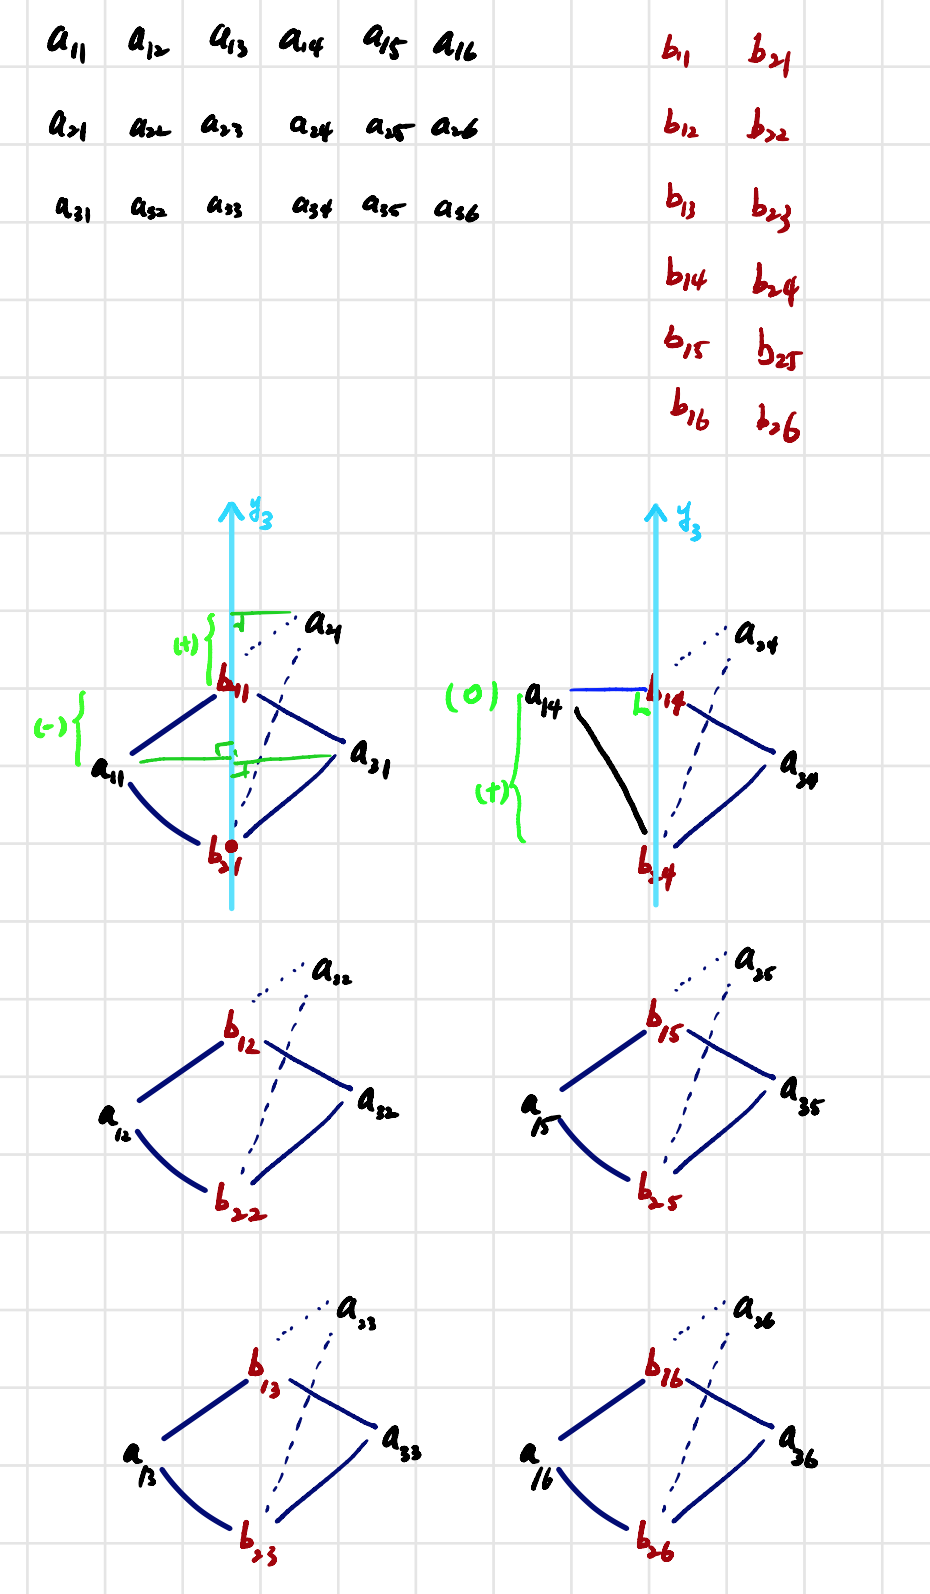
\includegraphics[scale=0.4]{1.png}
%\end{tcolorbox}

\section{Introduction}
This is no time for false equivalence: Today, neural networks have a wide range of applications. From unmanned aerial vehicles (UAV) to large language models (LLMs) which could have trillions of parameters. Consider an adversarial attack on the UAV, or a bug found in an LLM, e.g. it may give a false output to a certain set of inputs, is there a way to instantly recover the system without changing any of its functions? A possible solution is to generate infinitely many equivalent models so that a model that gives false output can be replaced immediately without a further cost to start over to train a new model.

Furthermore, inspired by \cite{yun2017global, blum1988training, judd1990neural}, consider the following question: can the neural network be trained to reach a global minimum on its loss surface? In a nutshell, is it possible to increase a well-trained model's performance?

%where the trained neural network already converged to a local minimum, then can the model be
%let a training set and a trained neural network be given where the trained neural network already converged to a local minimum, meaning given a positive real number $\epsilon>0$, then each sample $X_i$ in the given training set, there is $N\in\mathbb{N}$ such that for the number of epoch greater than $N$, the model is in the epsilon ball around the local minimum of the loss surface (i.e. its parameter space or moduli space).

Defining the following notions to describe the questions more precisely:
\begin{definition}
\textit{A neural network model (function) is converged} if it reaches one of local minima in its moduli space (i.e. loss surface).
\end{definition}

\begin{definition}
\textit{Two converged neural network models (functions) are equivalent} if they both give identical outputs on a fixed training set as the input.
\end{definition}

In other words, if the given model is denoted by $f_{\text{model}}$ which was trained by using samples in the training set $X$, since it is a function, consider a set of all $(f_{\text{model}},O)$, where $O$ is a neighborhood that contains $X$, then its equivalent model can be defined:
\begin{definition}
Two converged neural network models (functions) $f$ and $g$ trained within $O_1$ and $O_2$ are denoted by pairs $(f,O_1)$ and $(g,O_2)$. Furthermore, $(f,O_1)$ and $(g,O_2)$ are equivalent, if there exists an open set $O\subset O_1 \cap O_2$ containing $x$ such that $f(x)=g(x)$ when $f$ and $g$ are restricted to the open set $O$.
\end{definition}
\begin{proposition}\cite{tu2011manifolds}
The set of equivalent functions of $f$ is an equivalent class.
\end{proposition}


To use random matrix theory to study the eigenvalue distribution of the model, or to study the dynamics between the distributions of input and the distributions of the model, it takes time to generate samples of trained models. Not only that, if models are trained parallel, then they could not always be equivalent given there are multiple local minima. Hence, is it correct to collect models as samples to find their distribution or their eigenvalue distribution if they are not equivalent?

Hence, here is the \textbf{the essential question} that answered by this paper: \textbf{For any given neural network model}, is there a way to generate (infinitely many) equivalent models of a given (trained) model and \textbf{each generated equivalent model can have non-trivial feedback gradients during the training mode using back-propagation, and the generated equivalent models can give different output compared the given model when the input is out-of-sample}?

In other words, let $f$ be the given converged model that is trained using samples in the set $X$. Then, the goal is to find an equivalent converged $F$ in the equivalent class of $(f,O_1)$ such that
\begin{itemize}
\item[(i)] $F(x)=f(x), \forall x\in X$, 
\item[(ii)] there exists a set $X'$ that are not measure zero and $X'\neq X$ such that 
$$\mathbb{E} \left[ F(X') \right] \neq \mathbb{E} \left[ f(X') \right] \text{ and, }$$
\item[(iii)] The weights of the converged $F(x)$ are not an affine images of the weights of the converged $f(x)$ so that $F(x)$ can have non-trivial gradients while running gradient descent and back-propagation algorithm on it using a new training set to reach a new local or global minimum.
\end{itemize}

With the condition $(ii)$, $F$ cannot be a trivial composition of functions, e.g. $g^{-1}\circ g\circ f$, and with the condition $(iii)$, the weights of the converged $F$ cannot be an affine transformation of the converged $f$. 

It is necessary to ask this question so that the trained model can be understood better to a point that the distribution of its weights can be studied using random matrix theory, and if all the other equivalent models can be derived instantaneously, then this can be considered an alternative to apply quantum computing to find all those equivalent solutions in parallel.

If a model can be replaced by another equivalent model, then the other model might be at the different point on the loss surface, and the barrier between the local minimum to the nearest lower local minimum might have a lower height or in some better case with a negative height, meaning the model can be trained to a better model with a smaller error by using a new set of training data to descent to that lower local minimum. Hence, it is also sufficient to ask the question: how to find equivalent models of a given trained model? If the answer to this question is unknown, suppose a converged model cannot distinguish the fake data generated by an adversary model from the true data, or if a model needs to go through a debugging process for some false classified input, then the model not only has to be retrained, but it cannot be justified if it is the best solution due to the process to reach the solution is random. 

Thus, on the contrary, if its equivalent converged models can be found immediately after a short period of time of training using using a new training set such as the input generated by adversarial models, then chances are, \textbf{within the set of equivalent converged models, there might exist a converged model} that will not take the fake input or falsely classified a corner case. 

\section{Hyperbolic-length Product}

%To introduce the algorithm, it is natural to start to build up the concept and tools from the Euclidean space. In Euclidean space, equivalent models of a trained model can be obtained by redefining matrix multiplication using Euclidean distance $d_E(x,y)=\vert x-y\vert$ for all $x, y\in\mathbb{R}$. For instance, let $A$ be in $\mathbb{R}^{n\times m}$, $B$ be in $\mathbb{R}^{d\times m}$, and their entries are denoted by $a_{ki}$ and $b_{li}$ where $k\in\left\lbrace 1,...,n\right\rbrace$, $l\in\left\lbrace 1,...,d\right\rbrace$, and $i\in\left\lbrace 1,...,m\right\rbrace$. Then, $\left( A B^t\right)_{kl}=\sum\limits_{i=1}^m a_{ki}b_{il}$.

%Instead of using matrix multiplication, a new operation using Euclidean distance is defined in the following:
%$$
%\left( A\odot_{E} B^t \right)_{kl}:= \sum\limits_{i=1}^m d_{E} \left( a_{ki} , b_{il} \right).
%$$

%Now, let the above $A$ and $B$ be any two matrices that need to be multiplied in a given model that already converges under the above new operation $\odot_{E}$ between matrices $A$ and $B$. Then by adding a real number $\alpha$ to $A$ and $B$, infinite many equivalent models can be derived, since
%$$
%\left( \left( \alpha + A \right) \odot_{E}\left( \alpha+ B^t \right)\right)_{kl} := \sum\limits_{i=1}^m d_{E} \left(\alpha + a_{ki} ,\alpha + b_{il} \right) = \sum\limits_{i=1}^m d_{E} \left( a_{ki} ,  b_{il} \right) = \left( A\odot_{E} B^t\right)_{kl}.
%$$
%In other words, the original given model is unchanged. This operation results in a translation of the loss surface.

Every entry of the matrices $A\in\mathbb{R}^{n\times m}$ and $B \in\mathbb{R}^{d\times m}$ can be embedded into the upper half-plane $\mathbb{H}^2$. That is, the entries of $A$ and $B$ become complex numbers with positive imaginary part: $a_{ki}\in\mathbb{H}^2$ and $b_{il}\in\mathbb{H}^2$.

The necessary condition to use hyperbolic geometry and Kleinian groups is that since that hyperbolic geometry can also reach the goal that to generate infinitely many equivalent models, and Kleinian groups are isometry group that preserved not only hyperbolic lengths, but angles which can work as the symmetric group of the space, and to act on geometric objects in the space to do rigid transformation.

Furthermore, the sufficient condition to apply hyperbolic geometry and Kleinian groups is that instead of linear transformations, linear fractional transformations (which is determined by elements in the Kleinian group) can provide non-linear and hence non-trivial feedback in back-propagation. Though it is possible to develop a similar algorithm on other Riemannian manifold that has an automorphism group and if the group elements can also preserve angles and distance, hyperbolic geometry with Kleinian groups might be the easiest example that can be computable, but give non-trivial feedback in back-propagation.


Define a new binary operation between $A$ and $B$ using hyperbolic length on the upper-half plane $\mathbb{H}^2$\cite{beardon2012geometry}:
$$
\left( A\odot_{\mathbb{H}^2} B^t \right)_{kl} :=\sum\limits_{i=1}^m d_{\mathbb{H}^2} \left( a_{ki} , b_{il} \right).
$$

Then on the upper-half plane, the projective special linear group $\text{PSL}(2,\mathbb{R})$ is its automorphism group. Furthermore, elements of the group are conformal mapping that preserve not only angles but hyperbolic distance. Hence, $\text{PSL}(2,\mathbb{R})$ is also the isometry group of the upper-half plane.


To derive an equivalent model, take any $M\in \text{PSL}(2,\mathbb{R})\setminus\left\lbrace \text{id}\right\rbrace$, then there exists an isomorphism to map $M$ to a linear fractional (M\"{o}bius) map $T_M(z)=\frac{az+b}{cz+d}, a,b,c,d\in\mathbb{R},z\in\mathbb{C}$.
\begin{definition}[Hyperbolic-length product]
Define \textit{the hyperbolic-length product} is the following new operation:
$$
\left( T_M(A) \odot_{\mathbb{H}^2} T_M(B^t)\right)_{kl} := \sum\limits_{i=1}^m d_{\mathbb{H}^2} \left(T_M \left( a_{ki} \right) ,T_M\left( b_{il}\right) \right).
$$
\end{definition}
\begin{definition}
Let $W$ be a neural network model and assume $W$ converged already with the hyperbolic-length product implemented. Then with the above notations, the orbit of $W$ of the given weights $\left\lbrace a_{ki},  b_{il}\right\rbrace$ (points in the hyperbolic space) is the set:
$$
\left\lbrace T_M(a_{ki}) \right\rbrace \cup \left\lbrace T_M(b_{il}) \right\rbrace
$$
for all $M\in \text{PSL}(2,\mathbb{R})$, and for all $k\in\left\lbrace 1,...,n\right\rbrace$, $l\in\left\lbrace 1,...,d\right\rbrace$, and $i\in\left\lbrace 1,...,m\right\rbrace$.
\end{definition}
\begin{proposition}
With the above notations, then the newly defined product is an invariant:
$$
\left( T_M(A) \odot_{\mathbb{H}^2} T_M(B^t)\right)_{kl} = \sum\limits_{i=1}^m d_{\mathbb{H}^2} \left(T_M \left( a_{ki} \right) ,T_M\left( b_{il}\right) \right)
=  \sum\limits_{i=1}^m d_{\mathbb{H}^2} \left( a_{ki}  , b_{il} \right)  =\left( A\odot_{\mathbb{H}^2} B^t\right)_{kl}.$$
\end{proposition}
\begin{proof}
This result follows immediately from the property of the M\"{o}bius mapping $T_M$ when it is corresponding to a matrix $M$ in the projective special linear group $\text{PSL}(2,\mathbb{R})$, then $T_M$ is an isometry under the hyperbolic metric.
\end{proof}
Let $\mathbb{B}^2:=\left\lbrace z\in\mathbb{C} : \vert z \vert <1\right\rbrace$ be the Poincare's disc and $\Psi$ be the Cayley's transformation $\Psi: \mathbb{H}^2 \to \mathbb{B}^2$. Then, $\Psi\left( T_M(z)\right)=\frac{a'z+b'}{c'z+d'}$ where $a',b',c',d'\in\mathbb{C},z\in\mathbb{C}$.

\begin{proposition}
With the above definition and proposition, then the value of the product has the same value when the points $a_{ki}$ and $b_{il}$ are sent to Poincare's disc:
$$
\left( T_M(A) \odot_{\mathbb{H}^2} T_M(B^t)\right)_{kl} = \sum\limits_{i=1}^m d_{\mathbb{H}^2} \left(T_M \left( a_{ki} \right) ,T_M\left( b_{il}\right) \right)
=  \sum\limits_{i=1}^m \rho_{\mathbb{B}^2} \left(\Psi \left(T_M \left( a_{ki} \right)\right) ,\Psi\left( T_M\left( b_{il}\right) \right)\right) .$$
\end{proposition}
\begin{proof}
Since for each $z_1,z_2\in\mathbb{H}^2$, $d_{\mathbb{H}^2}(z_1,z_2)=\rho_{\mathbb{B}^2}(\Psi(z_1),\Psi(z_2)).$
\end{proof}

The 2-dimensional hyperbolic-length product can be generalized to $n$-dimension\cite{MR1138441, MR725161, beardon2012geometry, MR2402415, MR4221225, MR1893917}, for $n\geq 3$. Let $A, B$ be embedded into $\mathbb{H}^n, n\geq 3.$
\begin{definition}[Hyperbolic-length product]
Define \textit{n-dime the hyperbolic-length product} is the following new operation:
$$
\left( T_M(A) \odot_{\mathbb{H}^n} T_M(B^t)\right)_{kl} := \sum\limits_{i=1}^m d_{\mathbb{H}^n} \left(T_M \left( a_{ki} \right) ,T_M\left( b_{il}\right) \right).
$$
\end{definition}
This $n$-dimension result could be useful for applying the hyperbolic-orbit algorithm to any trained models that were trained without implementing the hyperbolic-length product during the training.
Likewise, for higher dimensions, the hyperbolic-length product is also an invariant:
\begin{proposition}
With the above notations, then the newly defined product is an invariant:
$$
\left( T_M(A) \odot_{\mathbb{H}^n} T_M(B^t)\right)_{kl} = \sum\limits_{i=1}^m d_{\mathbb{H}^n} \left(T_M \left( a_{ki} \right) ,T_M\left( b_{il}\right) \right)
=  \sum\limits_{i=1}^m d_{\mathbb{H}^n} \left( a_{ki}  , b_{il} \right)  =\left( A\odot_{\mathbb{H}^n} B^t\right)_{kl}.$$
\end{proposition}

The question that aimed to solve by using this algorithm was mentioned in the first section. The goal is to replace matrix multiplication with a caveat that the situation mostly does not include finding inverses.

Let a converged model $W$ and a training set $X$ be given. The goal is to find its converged equivalences.

\begin{definition}
Hyperbolic-orbit Algorithm is an algorithm that implements hyperbolic-length products to replace matrix products.
\end{definition}
The following section introduces the hyperbolic-orbit algorithm. 


%\item[Case 1] $W$ was trained. A special case when $d=2$ for the matrix $B$:
%\begin{itemize}
%\item[Step 1] Start with dimension $3\times d$ for embedding $A$ and $B$: each $l$-th column vector in the matrix $B$ is embedded in parallel to the third axis of $\mathbb{H}^3$, denoted by $y^3$ in the following example.

%\item[Step 2]
%\begin{itemize}
%\item For $k=1$ to $k=n$ and fix $l$ at $l=1$.
%\begin{itemize}
%\item[(i)] If $a_{ki}b_{il}=0$, then map the edge $(a_{ki},b_{il})$ to a plane that is orthogonal to $y^3$-axis and has a zero projection to $y^3$-axis. 
%\item[(ii)] If $a_{ki}b_{il}>0$, then map the edge $(a_{ki},b_{il})$ to a plane that is parallel to $y^3$-axis and has a positive projection with an absolute hyperbolic value equal to $a_{ki}b_{il}$ to $y^3$-axis. 
%\item[(iii)] If $a_{ki}b_{il}<0$, then map the edge $(a_{ki},b_{il})$ to a plane that is parallel to $y^3$-axis and has a negative projection with an absolute hyperbolic value equal to $a_{ki}b_{il}$ to $y^3$-axis. 
%\end{itemize}

%\item For $k=1$ to $k=n$ and fix $l$ at $l=2$.
%\begin{itemize}
%\item[(i)] Let $b_{i2}$ have the same $y^1$ and $y^2$ coordinates as $b_{i2}$.
%\item[(ii)] If $a_{ki}b_{i2}=0$, then move $b_{i2}$ along its $y^3$ coordinate such that the edge $(a_{ki},b_{il})$ has a zero projection to $y^3$-axis. 
%\item[(iii)] If $a_{ki}b_{i2}>0$, then move $b_{i2}$ along $y_3$-axis such that the edge $(a_{ki},b_{il})$ has a positive projection with an absolute hyperbolic value equal to $a_{ki}b_{il}$ to $y^3$-axis. 
%\item[(iv)] If $a_{ki}b_{i2}<0$, then move $b_{i2}$ along $y_3$-axis such that the edge $(a_{ki},b_{il})$ has a negative projection with an absolute hyperbolic value equal to $a_{ki}b_{il}$ to $y^3$-axis. 
%\end{itemize}
%\end{itemize}
%\end{itemize}
\section{Hyperbolic-orbit Algorithm}

Let $A$ and $B$ be \textbf{any} two matrices in \textbf{any} converged neural network model $f$ that was implemented with a matrix multiplication between $A$ and $B$. \textbf{It is prefer to let at least one of $A$ and $B$ to be a weight matrix (tensor) of the model $f$. In general, $A$ could be any weight matrix (tensor) in any given neural network $f$, and let $B$ be the identity matrix (tensor).}
\begin{itemize}
\item[Case 1] Let $f$ be \textbf{any} neural network model that was trained.

\begin{itemize}

\item[Step 1]
Embed entries of $AB$ to $\mathbb{H}^2$ by mapping each column vector of $AB$ to a line parallel to $y^2$-axis without any overlapping on coordinates so that each pare circles does not have any overlap to each other. Denote the embedding function by $\phi$.

\item[Step 2] Constructing an invertible matrix $C$ by taking points on a line that is parallel to $y^2$-axis without any overlapping in their coordinates and forming edges to its corresponding set of embedded entries from the column vector in $AB$--the correspondence is determined by matrix multiplication $(AB)C$. (See the following figure for an example when $\phi(AB)$ and $C$ are 4 by 4.)
\item[Step 3] Measuring all the hyperbolic length of edges in each $K_{n,d}$-graph (composed by vertices on the hyperbolic circle and the line that passes through its center), and sum all the lengths in each $K_{n,d}$-graph to make an entry of matrix $M$.

\item[Step 4] Pick an element $g\in\text{PSL}(2,\mathbb{R})$, derive a linear fractional mapping from $g$, and denote it by $T_g(z)=\frac{az+b}{cz+d}, z\in\mathbb{H}^2$. 
\item[Step 5] Apply $T_g$ to every entry $z$ of $\phi(AB)$ and $C$ to map every entry (could be trillions) of both matrices to their images $T_g(z)$ to derive the new weights of the given model, i.e. to derive an equivalent model.

\item[Step 6] Apply gradient descent back-propagation algorithm on the whole model to reach a new local or global minimum with a new training set.
\end{itemize}


\item[Case 2] $W$ was not trained.
\begin{itemize}
\item[Method 1] Treat $W$ as trained and reduce it to either case 1.
\item[Method 2] Train $W$ without using hyperbolic-length product till it converges, then treat it as trained, i.e. again, apply methods of case 1.
\item[Method 3] Implement the hyperbolic-length product into $W$ directly.
\begin{itemize}
\item[Step 1] The selected matrices $A$ and $B$ can be embedded freely to hyperbolic space as long as the hyperbolic-length product can work properly in the usual training process. Denote the embedding images by $\phi(A)$ and $\phi(B)$.
\item[Step 2] The dimension of hyperbolic space could start with two dimensions to optimize the memory usage. 
\item[Step 3] Pick an element $g\in\text{PSL}(2,\mathbb{R})$, derive a linear fractional mapping from $g$, and denote it by $T_g(z)=\frac{az+b}{cz+d}, z\in\mathbb{H}^2$. 
\item[Step 4] Apply $T_g$ to every entry $z$ of $\phi(A)$ and $\phi(B)$ to map every entry (could be trillions) of both matrices to their images $T_g(z)$ to derive the new weights of the given model, i.e. to derive an equivalent model.

\item[Step 5] Apply gradient descent back-propagation algorithm on the whole model to reach a new local or global minimum with a new training set.
\end{itemize}
\end{itemize}
\end{itemize}
\textbf{Remark 1:} The algorithm not only preserves the hyperbolic lengths, but the angle between its angle to the $y^2$ axis--this is the reason to use conformal mapping $T_g$. Hence, in Case 1 and Case 2, the hyperbolic-product could actually preserve the information of negative values, and one more layer of operation, i.e. subtraction, could be easily implement with the algorithm using the projection of the hyperbolic length to the $y^2$-axis. That is, it can have a zero, positive, or negative projection. Furthermore, the amount and sign of each of these projections (could be trillions) are preserved when $T_g\in\text{PSL}(2,\mathbb{R})$ is applied to these (trillions) of weights, and the choice of $T_g$ is infinitely many--images of all of the choices of $T_g$ form the orbit of the model, and each image on the orbit gives an equivalent model.

\textbf{Remark 2:} Since it is possible that two entries in the matrix $AB$ have the same values. To design an invertible embedding, the following is an example of the embedding function $\phi: \mathbb{R}\to \mathbb{R\times \mathbb{R}\times \mathbb{H}^2}$:
$$
\phi(x_{ij})=(i,j,(ax+b)+ci)
$$
where $x_{ij}$ is the $i$-th row and $j$-th column from $AB$, and $a,b,c$ are some real numbers such that $(ax+b)+ci\in\mathbb{H}^2$.
\begin{figure}[H]
\caption{The computational graph of case 1.}
\centering
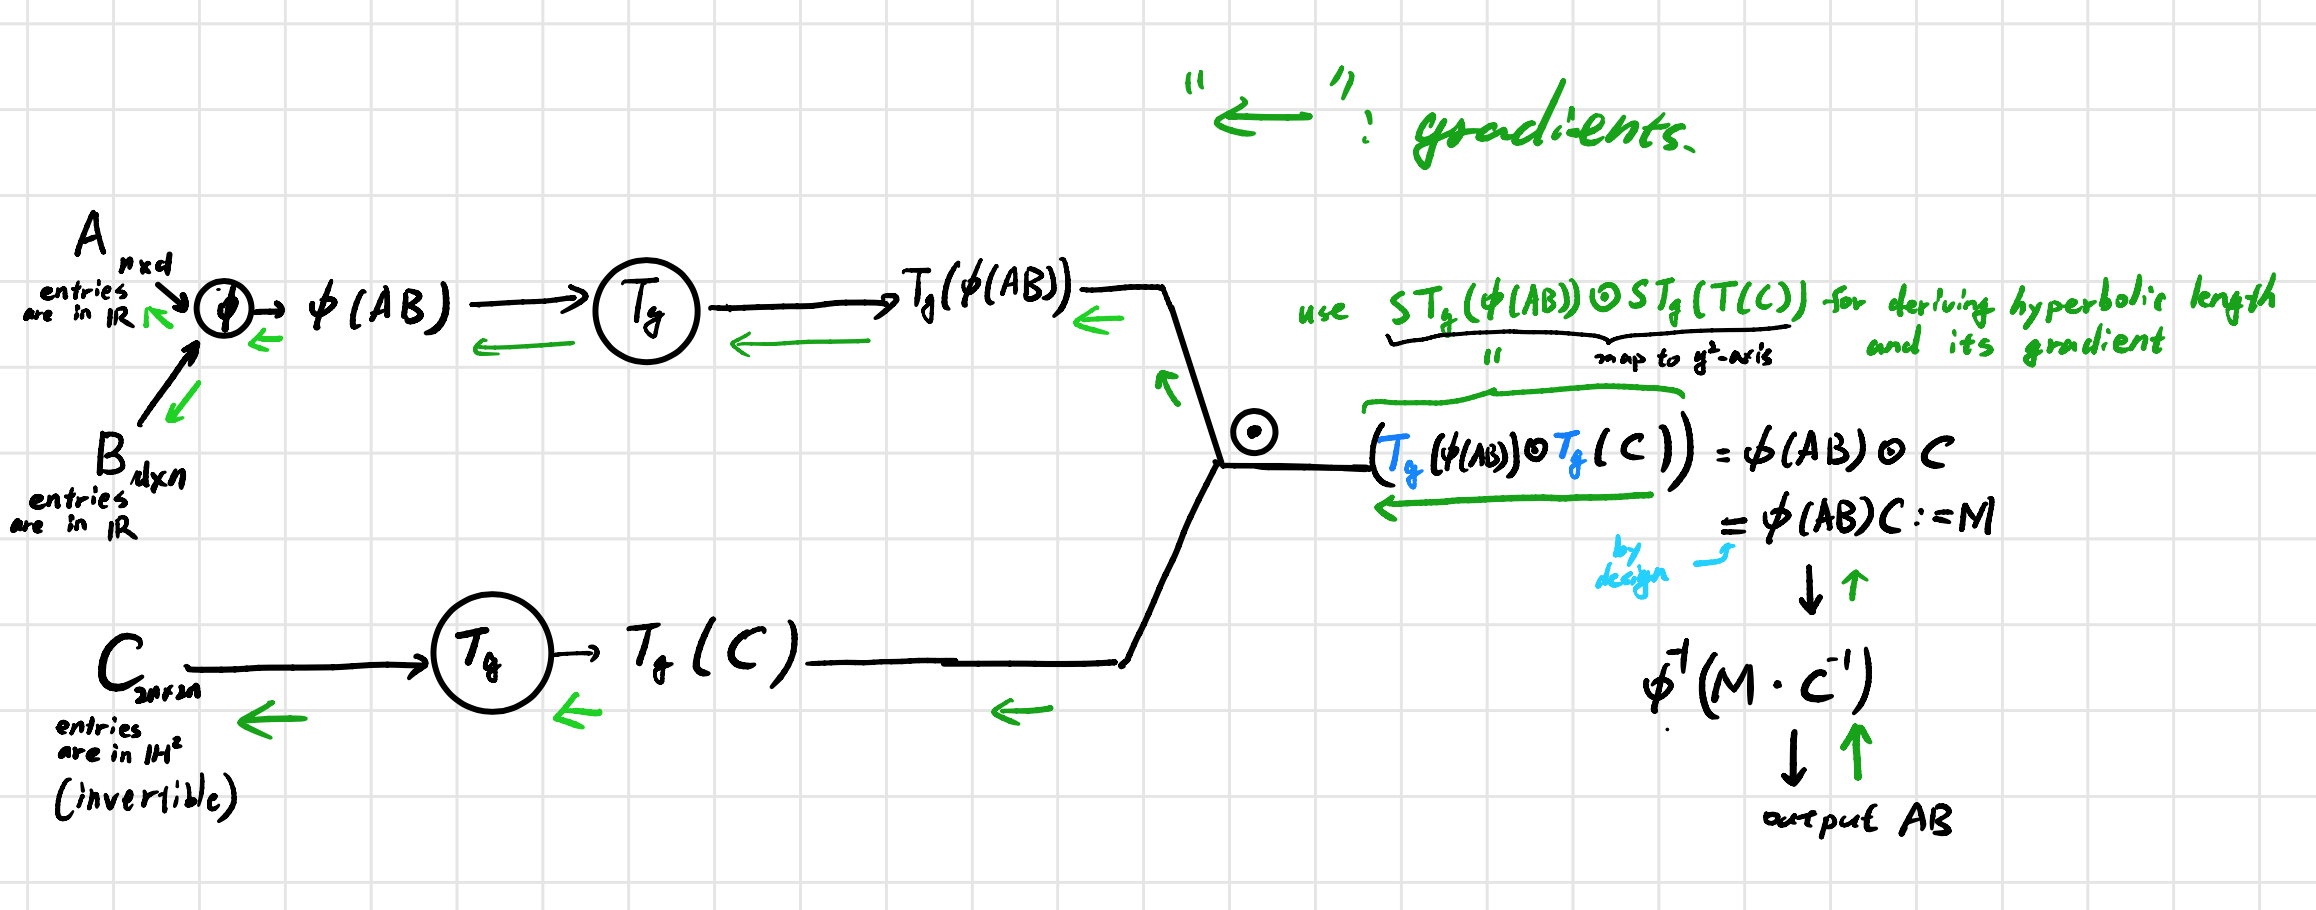
\includegraphics[width=0.8\textwidth]{8.png}
\end{figure}

\begin{figure}[H]
\caption{An illustration on how to embed \textbf{any} given product of matrices $AB$ in \textbf{any neural network models} to hyperbolic space $\mathbb{H}^2$.}
\centering
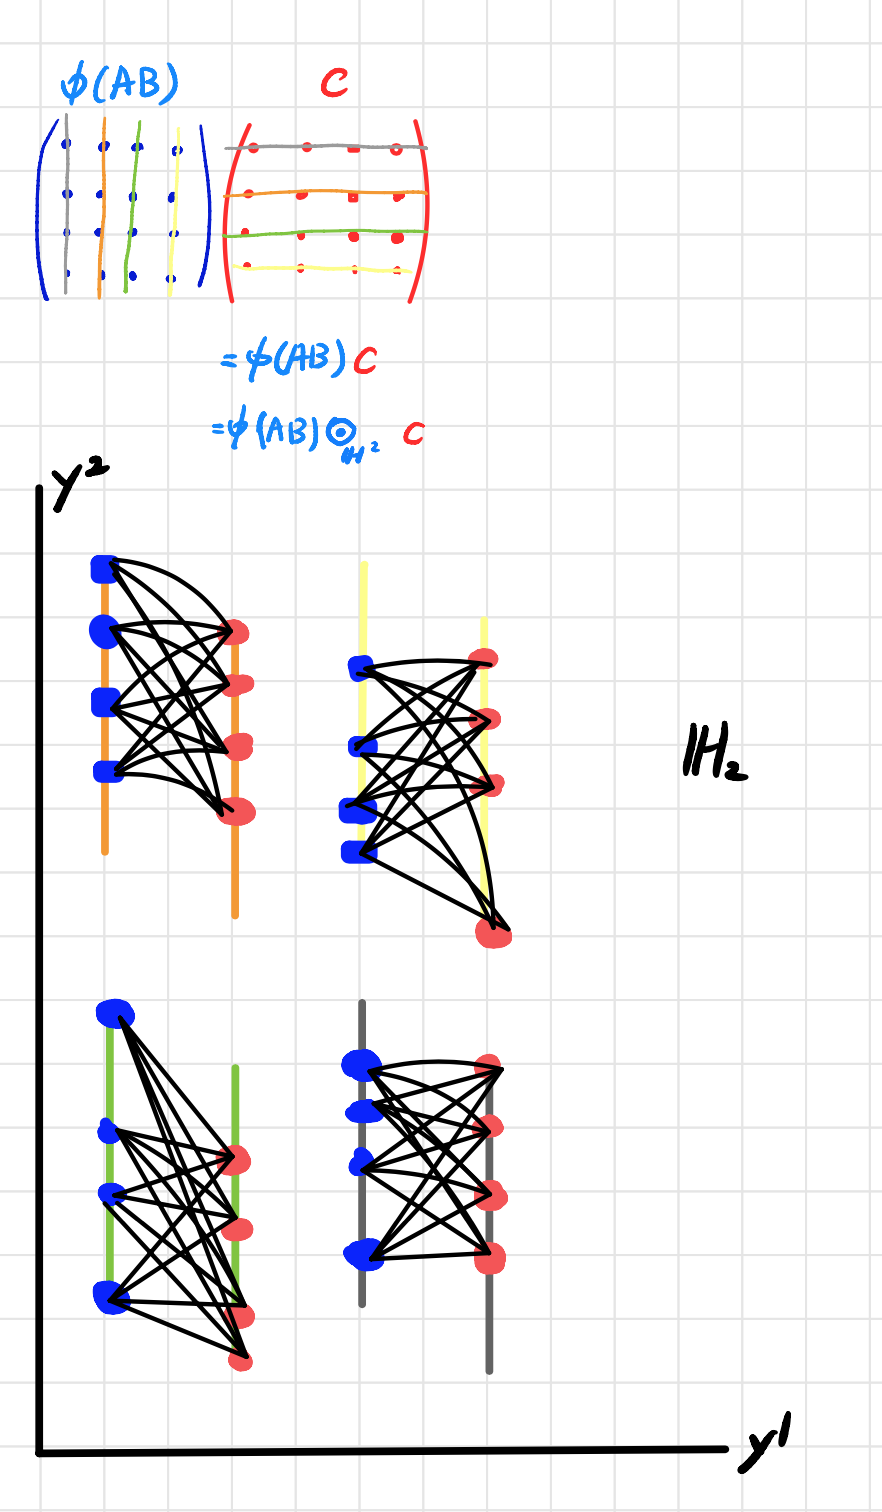
\includegraphics[width=0.8\textwidth]{9.png}
\end{figure}

\begin{figure}[H]
\caption{Gradients of the hyperbolic-length product.}
\centering
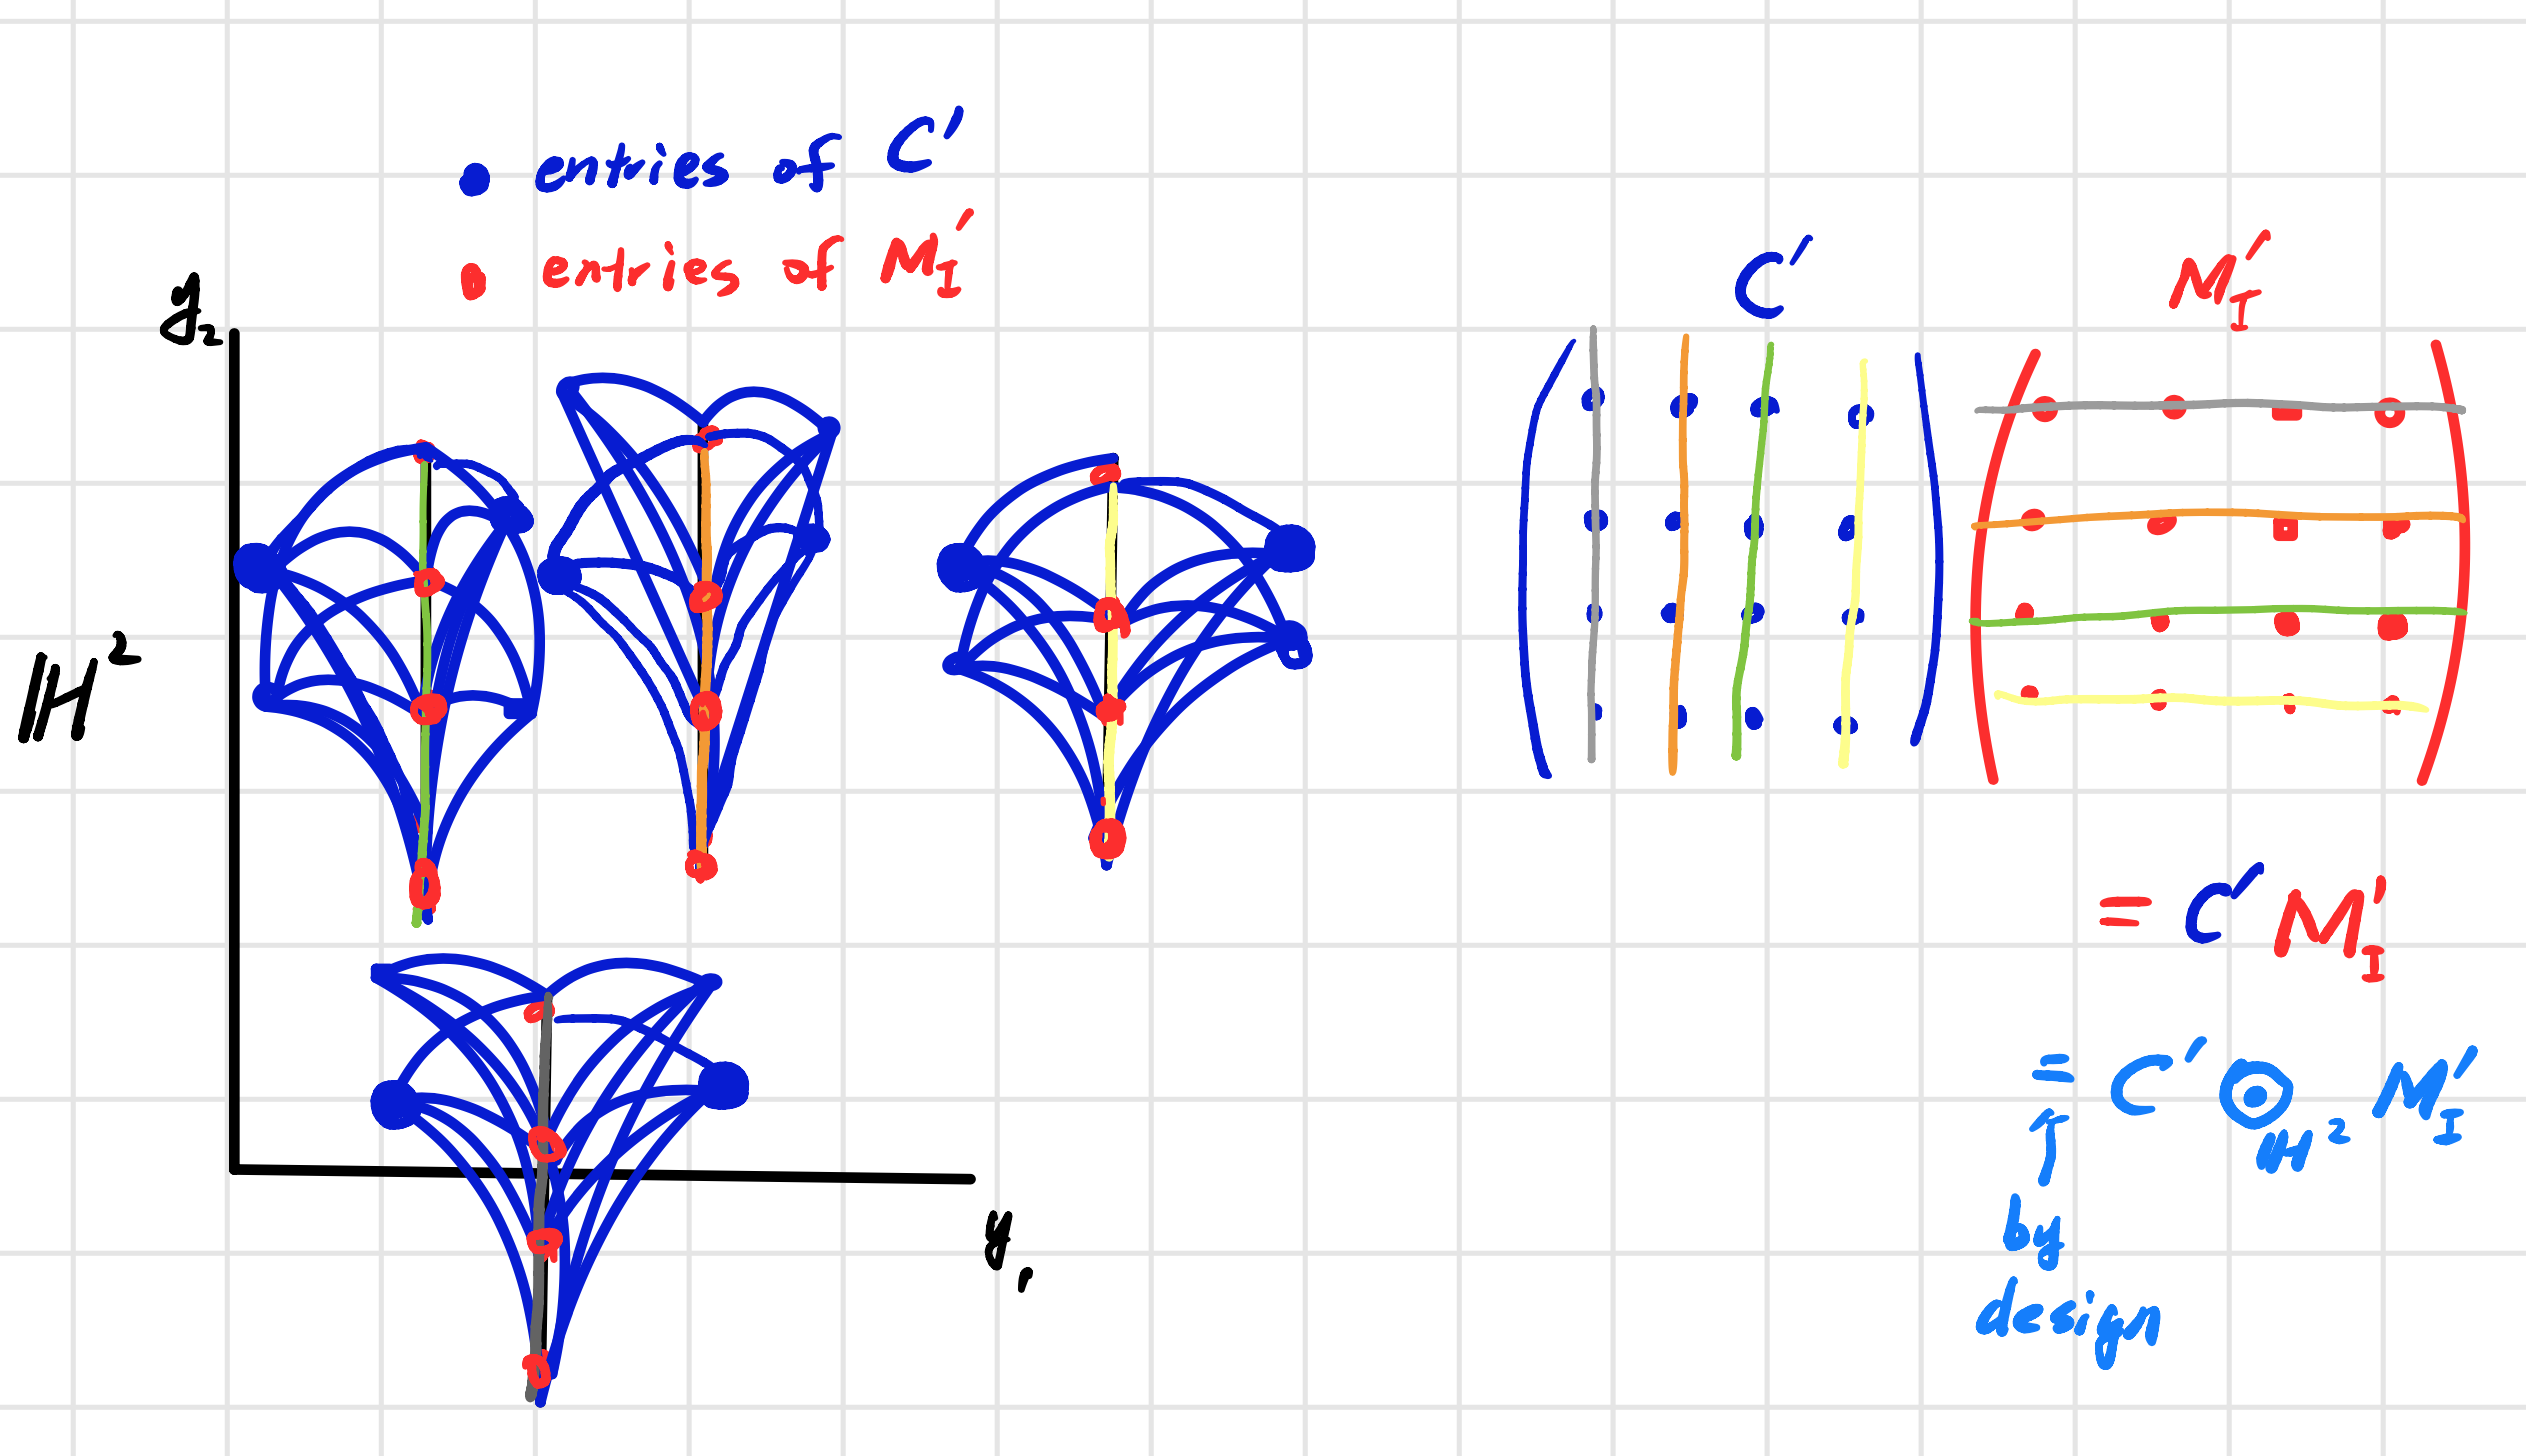
\includegraphics[width=0.8\textwidth]{6.png}
\end{figure}

\begin{figure}[H]
\caption{The computational graph of Case 2 when a hyperbolic-length product is implemented to the model directly before training.}
\centering
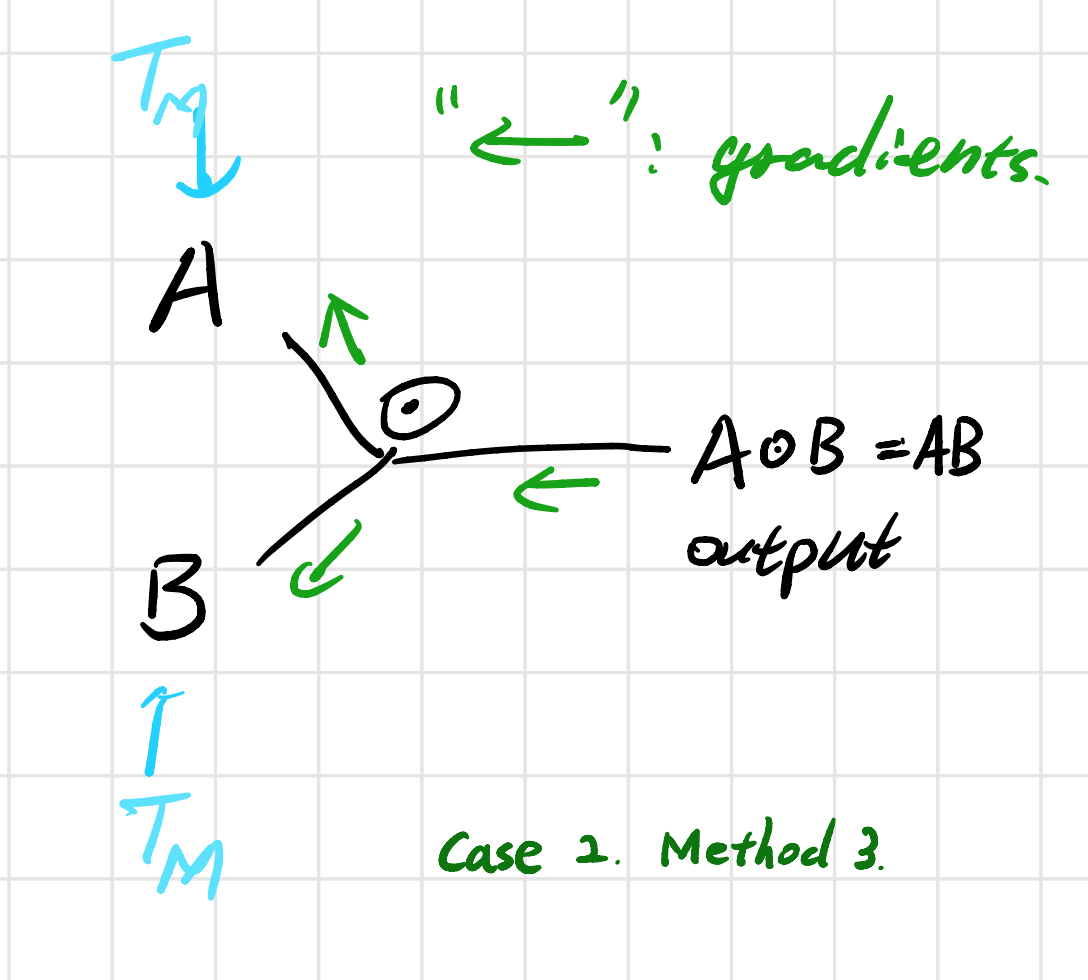
\includegraphics[width=0.8\textwidth]{5.png}
\end{figure}






\section{Examples}
\subsection{Self-attention mechanism in any transformer-based models with the hyperbolic-length product implemented before training}
All layers of a given neural network model can be implemented with the above hyperbolic-orbit algorithm. The following is an example when the hyperbolic-orbit algorithm is applied to the self-attention mechanism, i.e. transformer-based models.
Let $A=Q\in \mathbb{C}^{n\times d_q}$ and $B=K^t\in \mathbb{C}^{d_k\times n}$ in self-attention mechanism\cite{vaswani2017attention} using dynamic scaling factor $\beta$ (defined in our another work in progress), and by convention let $d_q=d_k$. Then, for each entry of the matrix $QK^T$, its denominator is a finite Poincar\'{e} series\cite{chuang2022hausdorff}, and its dynamic scaling factor (work in progress) is corresponding to the entropy of the system, e.g. a system could be words in an input string. 



%\subsection{Apply to models that were trained without using the hyperbolic-length product}
%Hyperbolic-orbit Algorithm can be implemented into any models that is trained in a traditional method immediately. Let $\Omega$ be a model that is trained without using hyperbolic-length products. Once the matrix multiplication between two matrices called $A$ and $B$ within $\Omega$ is chosen to be replaced with hyperbolic-length product, the matrices $A\in\mathbb{R}^{n\times m}$ and $B \in\mathbb{R}^{m\times d}$ can be easily embedded into $\mathbb{H}^2$.

%In matrix $A$, the $i$-th column which has $n$ entries, and in matrix $B$, the $i$-th row which has $d$ entries will have $n\times d$ products and this gives $n\times d$ equations to determine where to embedded $a_{ki}$ and $b_{il}$.

%Denote the images of $a_{ki}$ and $b_{il}$ in $\mathbb{H}^2$ using $a_{ki}'$ and $b_{il}'$.
%The following embedding algorithm can test if the hyperbolic-orbit algorithm is applicable.
%For each i in 1,...,m, and for each l in 1,...,d: Consider hyperbolic circles center at $b_{il}'$ with radii $d_{\mathbb{H}^2}(a_{ki}', b_{il}' )=a_{ki}b_{il} $, and k from 1 to n.
%Consider hyperbolic circles center at $b_{ij}'$ for each $j\neq l$  with radii $d_{\mathbb{H}^2}(a_{ki}', b_{ij}' )=a_{ki}b_{ij} $, and k from 1 to n.
%If for each $k$, each pair of hyperbolic circles that are corresponding to the same k, one has radius $d_{\mathbb{H}^2}(a_{ki}', b_{il}' )$ and the other has radius $d_{\mathbb{H}^2}(a_{ki}', b_{ij}') $ has an interception, then do the next $j$ of $b_{ij}'$.
%Finally, if there exist interceptions in the above process for all i, then $A$ and $B$ can be embedded into $\mathbb{H}^2$ and use the hyperbolic-orbit algorithm to replace matrix multiplication.

%After implementing the hyperbolic-length product and hyperbolic-orbit algorithm to the trained model, with the same training set that trained the model, the new modified model will give exactly the same output. The only distinction will happen only when the old and new model were fed in samples that were out of the training set.

%The above two examples show that implementing the hyperbolic-orbit algorithm before training is way easier than the other way around. To solve this problem, instead of embedding $A$ and $B$ into 2-dimensional hyperbolic space, hyperbolic spaces in higher dimensions could be the solution, since for each $n\geq 3$, $\mathbb{H}^n$ has an isometry group. This is the sufficient condition for generalizing 2-dimensional hyperbolic-length products to n-dimension.

\section{Empirical Results}
Work in progress. The off-line code could be finished after the quals.

\section{Discussion}
In Case 1, since each step from step 1 to step 3 is invertible, after these operations, hyperbolic-length product can be applied to $M_I'$ and $C'$, then apply all the inverses and restrictions to back to $AB$, so the output is also unchanged, but the orbit of the neural network can be found using the above hyperbolic-orbit algorithm.

Furthermore, the isometry group of $\mathbb{H}^n$ is a group of M\"{o}bius mapping, hence its group elements preserve not only hyperbolic length but angles, thus the information of the sign of each $a_{ki}b_{il}$ could be preserved.

With the hyperbolic-orbit algorithm, it is possible to find an appropriate M\"{o}bius mapping that is corresponding to $M\in\text{PSL}(2,\mathbb{R})$ such that training a 3-node neural network become not necessarily NP-hard in \cite{blum1988training}. Further, if every layer of a given converged neural network is implemented with the hyperbolic-orbit algorithm introduced in this paper, by combining with perturbations and parallel computing, the steepest descent path toward the global minimum could be designed. 

The algorithm introduced by the paper can help to save training time for parallel computing in the ensemble method, that is, instead of starting over from the beginning to train $N'$ models in parallel, $N'\in\mathbb{N}$, the training can start with $N'$ converged models that are equivalent to the given converged model are converged to different minima in the moduli space using a new training set.




Since the moduli space of any given converged neural network is determined by the range of images of $T_g\in\text{PSL}(2,\mathbb{R})$, i.e. its orbits. By choosing a different set of isometries to form $T_g$ could determine a different fundamental group and a corresponding hyperbolic surface $M$. The set of equivalence classes of the metrics on the surface $M$ could be investigated using its corresponding moduli space of hyperbolic surfaces (which is also known as the Teichm\"{u}ller space). There is a unique K\"{a}hler-Einstein metric \cite{cheng1980existence}, and the geometry and topology of loss surface of any given converged neural network are determined by the weights of that neural net, the geometry and topology of the family loss surfaces could be investigated using recent results of K\"{a}hler-Einstein metric.

The range of $T_g\in\text{PSL}(2,\mathbb{R})$ determines the range of orbits of a given converged neural network. The number of possible ranges are determined by the hyperbolic surface that is determined by the group generated by all $T_g$ that were used to map the orbits. The number of these hyperbolic surfaces could also be enumerated using the method introduced in\cite{chuang2015implications} which gives not only a systematic way to enumerate these hyperbolic surfaces, but also can be used to enumerate the number of ways to transform any given neural net on its orbit by machines in a systematically.

Since each $T_g$ is a continuous open mapping, there exists an open set $O$ to cover all images of the weight tensor of a given model $f$. By studying the topology and geometry of the moduli space that this open set $O$ can move over, the topology and geometry of the loss surface could be investigated. In other words, this paper also demonstrates a correspondence between the moduli space of $T_g$, i.e. the Teichm\"{u}ller space, and the loss surface (landscape) of any given model.


Furthermore, this algorithm could also be applied for non-linear encryption. For instance, the cardinality of the orbit of $A$ and $B$ is infinite, thus there are infinitely many ways to encrypt messages in A or $B$. Let message be embedded in $(T_1(A)\odot_{\mathbb{H}^n}T_1(B))^N$ by using $T_1$. Then the message can only be deciphered if the receiver knows the two correct isometries $T_3$ and $T_2$ and a large integer $N$ as keys to decode two encrypted matrices: $T_2(B)$ and $T_3(A)$ to reconstruct the message in $(T_1(A)\odot_{\mathbb{H}^n}T_1(B))^N$ using $(T_1(A)\odot_{\mathbb{H}^n}T_1(B))^N = (A\odot_{\mathbb{H}^n}B)^N$. The meaning of the matrix $B$ is not only a lock, but it can obfuscate the frequency of characters used in the message in a random method. Since $T_2$ and $T_3$ are linear fractional, i.e. they have the form $\frac{az+b}{cz+d}$, thus the keys only need eight real numbers plus a large integer.

Compared to starting over to train a new model, the advantage of this hyperbolic-orbit algorithm is that it can preserve most of the learned features in the model while reaching a new local or global minimum. Since the loss surface is changed by the hyperbolic-orbit algorithm (since the weights of the model were mapped to new images in the hyperbolic space by a fractional linear mapping), the old local or global minimum might be mapped to a hill or halfway up a mountain. Without using the hyperbolic-orbit algorithm, to train a converged model using new training set might take a long time with a large data set to move the model out of a local or global minimum and then move it to another minimum that can take care of not only the old training set but also the new training set. Using the hyperbolic-orbit algorithm, it is very likely that after using a small set of new data, the model can converge to a new minimum without losing features that it already learned, i.e. the model could give the same output if the input is from the old training set.


%\section{Limitation}
%The hyperbolic-orbit algorithm has a limitation when it is applied to case 2 if the model was trained. To show the limitation, consider an example where there are two points $a_1$, and $a_2$ from $A$, and two points $b_1$ and $b_2$ in $B$. In $\mathbb{H}^n, n\geq 3$, suppose the hyperbolic length between $b_1$ to $a_1$ and $b_2$ to $a_1$ are both zero, and the hyperbolic length between $b_1$ and $a_2$ is $L$. But, for $b_2$, the hyperbolic length between $b_2$ and $a_2$ is $2L$. If this happens, it might be possible to find an auxiliary invertible matrix $C$ and instead of applying hyperbolic-orbit algorithm on $A$ times $B$, applying it to $AB$ times $C$ and multiply the final result with $C$ inverse such that the matrix product $ABC$ is positive and does not have any case like the one mentioned in this section. %This is the starting point of designing case 1 in the algorithm

%If this case happen, then it might be able to solve by randomly embedding $A$ and $B$ to $\mathbb{H}^n$, then applying isometries of $\mathbb{H}^n$ to rotate those zeros to other points such that none of the entries in $A$ and $B$ are zeros before applying the hyperbolic-orbit algorithm.


%\item[Step 1] Start with dimension $n\times d$ for embedding $A$ and $B$.
%\item[Step 2] Without loss of generality, for each $i$, choose the entry $b_i1$ in the matrix $B$ to be embedded to $\mathbb{H}^{nd}$. Embedded all $a_{ki}$ for $i$ from 1 to $n$ that are related to $b_i1$ in the matrix multiplication $AB$ to $\mathbb{H}^{nd}$ in a way that each hyperbolic length $d_{\mathbb{H}^{nd}}(a_{ki},b_{i1})=a_{ki}b_{i1}$. Then, embed $b_{i2}$ by updating the coordinates of each $a_{ki}$ to satisfy the condition $d_{\mathbb{H}^{nd}}(a_{ki},b_{i1})=a_{ki}b_{i1}$ for all $k$. To update the coordinates of each $a_{ki}$, all $b_{i1}, b_{i2},...,b_{i(l-1)}$ are fixed, since there is no restriction on hyperbolic length between $b_{il}$ and $b_{il'}$ for all $l\neq l'$. However, after each change on the coordinates of each $a_{ki}$, the hyperbolic length $d_{\mathbb{H}^{nd}}(a_{ki},b_{i1})=a_{ki}b_{i1}, d_{\mathbb{H}^{nd}}(a_{ki},b_{i2})=a_{ki}b_{i2},...,d_{\mathbb{H}^{nd}}(a_{ki},b_{i(l-1)})=a_{ki}b_{i(l-1)}$ must be maintained.
%\item[Step 3] Repeat the same procedure for $l$ from 1 to $d$ for each $b_{il}$. After each iteration, increase $i$ by one.

%\begin{lstlisting}[language=iPython]
%<- #there shouldn't be quotation marks
%"""
%---------
%sin2_theta  = np.sin(theta)**2 - a + b
%"""
%import math
%import numpy as np
%from lib.analytical import csa
%MAS = math.degrees(math.acos(math.sqrt(1/3)))/360 * 2* math.pi + a -b
%\end{lstlisting}

\bibliographystyle{amsplain} % We choose the "plain" reference style
\bibliography{refs} % Entries are in the refs.bib file
\end{document}







